\chapter{Methodology \& Numerical Simulation}
\label{ch:numsim}

\section{The Purpose of Numerical Simulations}
\label{sec:numerical-purpose}

\section{The Mathematics of Numerical Simulations}
\label{sec:numerical-math}

\section{Computational Hydrodynamics}

\label{sec:hydrodynamics}

\section{The Athena++ Hydrodynamical code}
\label{sec:athenapp}

\section{Simulating CWB systems}

\subsection{Assumptions}

\section{Cooling in numerical simulations}

\subsection{Plasma cooling}

\subsection{Dust cooling}
\label{sec:dustcoolingmodel}

% Discuss dust cooling in brief, link to section in background, touch on lambda being dependent on 3 rather than 1 value

% Difficulties in dust cooling integral, faster method of doing this

A particular difficulty in precisely calculating the rate of cooling due to emission from dust is calculating the electron transparency, $h_e$.\footnote{The probability that an electron will embed in the dust grain and heat it, rather than pass through.}
$h_e$ can be computed via integration by parts, however due to this occurring in the main cooling loop, this results in a nesting of integrals, which can lead to extremely time-consuming computation for individual cells.
Initial tests using the integral method within a numerical simulation led to severe slowdown as processing time for cooling took up to 90\% of the overall processing time for each timestep.

Multiple options were considered for improving the performance of this routine.
Initially, a $\Lambda_d$ lookup table was considered, this consisted of a logarithmically spaced table of $\rho$, $a$, $T$ and $\Lambda_d$ values calculated by an implementation of the \cite{dwek_infrared_1981} prescription. 
A binary search for each parameter is performed, with the an offset being calculated for each parameter,

\begin{equation}
  P_{d}=\frac{P-P_{0}}{P_{1}-P_{0}} , 
\end{equation}

these offsets are then used to perform a trilinear interpolation to calculate $\lambda_d$ from the lookup table.

\begin{equation}
  \begin{split}
    \Lambda_{00} &=\Lambda_{000}\left(1-\rho_{d}\right)+\Lambda_{100} \rho_{d}, \\
    \Lambda_{01} &=\Lambda_{001}\left(1-\rho_{d}\right)+\Lambda_{101} \rho_{d}, \\
    \Lambda_{10} &=\Lambda_{010}\left(1-\rho_{d}\right)+\Lambda_{110} \rho_{d}, \\
    \Lambda_{11} &=\Lambda_{011}\left(1-\rho_{d}\right)+\Lambda_{111} \rho_{d}, \\
    \Lambda_{0} &=\Lambda_{00}\left(1-a_{d}\right)+\Lambda_{10} a_{d}, \\
    \Lambda_{1} &=\Lambda_{01}\left(1-a_{d}\right)+\Lambda_{11} a_{d}, \\
    \Lambda &=\Lambda_{0}\left(1-T_{d}\right)+\Lambda_{1} T,
  \end{split}
\end{equation}

%//TODO this needs a bit of sprucing, but makes sense
where 0 is the lookup table value lower than the parameters actual value, and 1 is the lookup table value greater than the parameters actual value.
This implementation was written in the form of a series of nested loops to utilise SIMD vectorisation to improve performance.

% Further optimisations

Whilst this method is significantly faster than calculating $\Lambda$ for each cell with an integration step, a $(100 \times 100 \times 100)$ lookup table requires \SI{32}{\mega B} of memory to store, and is much more time consuming to search through.
As such, eliminating complexity from the binary search and reducing the number of interpolations were identified as improvements to the 
These optimisations were made by simplifying the lookup table into a series of smaller lookup tables and relying on even logarithmic spacing of the lookup table to perform a calculation to determine the parameter indices, rather than performing a binary search.
Additionally, as $\rho$ and $a$ are invariant within the cooling loop, these parameter offsets are solved separately using a bilinear interpolation, while in the cooling sub-step loop, a separate linear offset is performed to find the temperature offset, solving to find $\Lambda_d$. These optimisations resulted in this method scaling significantly better, as there is a lower total number of calculations required as the number of sub-steps increases (figure \ref{fig:dust-opt-speedup}).

\begin{figure}
  \centering
  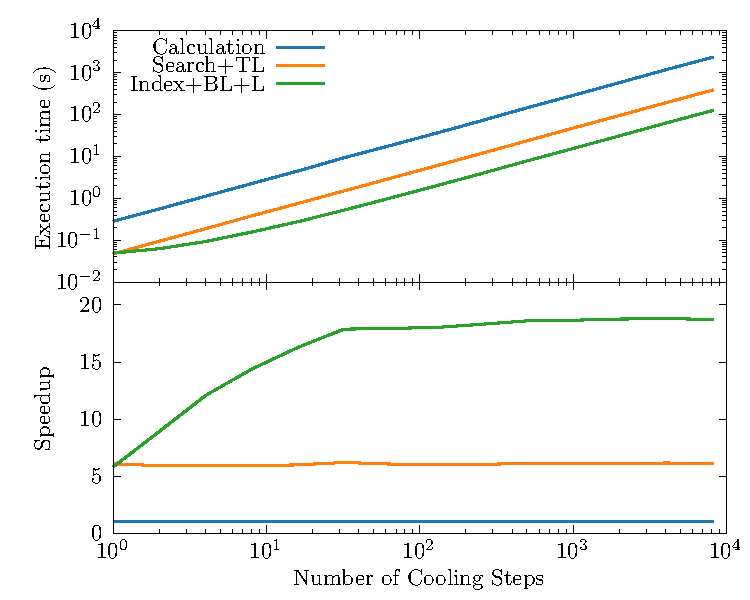
\includegraphics{assets/lambda-dust-speedup/lambda-dust-speedup.pdf}
  \caption[Dust lookup table methods comparison]{Comparison of execution time and speedup for lookup table methods.}
  \label{fig:dust-opt-speedup}
\end{figure}



% Approximations in that one paper, you know the one
The second method considered for solving the $h_e$ integral was using an approximation described by \cite{dwek_infrared_1981} where $h_e$ could be described by a series of equations:

\begin{equation}
  \begin{alignedat}{3}
    h_e(x^*) & = 1 ,                && ~~ x^* > 4.5, \\
    & = 0.37{x^*}^{0.62} , && ~~ x^* > 1.5 , \\
    & = 0.27{x^*}^{1.50} , && ~~ \text{otherwise,}
  \end{alignedat} \label{eq:electrontransparencyestimate}
\end{equation}

where $x^* = 2.71 \times 10^8 a^{2/3}(\si{\micro\metre}) /T$.
Whilst this is less accurate, especially in the region where one case ends and the other begins where the result begins to diverge, this method is multiple orders of magnitude faster.
Figure \ref{fig:graintransacc} shows these discrepancies, in the case where electron transparency begins to decrease the approximation is out somewhat significantly, as well as mid-way through the curve, whilst at temperatures below $10^6 \, \si{\kelvin}$ the approximation and integral methods are perfectly aligned.
As the grains grow hotter and the electron transparency reduces, the influence on the cooling rate due to incident electrons reduces quite drastically, meaning that extremely high accuracy is less important at these temperatures (figure \ref{fig:contribution-int-vs-est}).
The accuracy of the approximation method is also shown in figure \ref{fig:lambda-comp-int-vs-est}, the estimated value for $\Lambda_d$ closely matches the integrated value aside from the smallest dust grains at very high temperatures $T>\SI{6e8}{\kelvin}$.


\begin{figure}
  \centering
  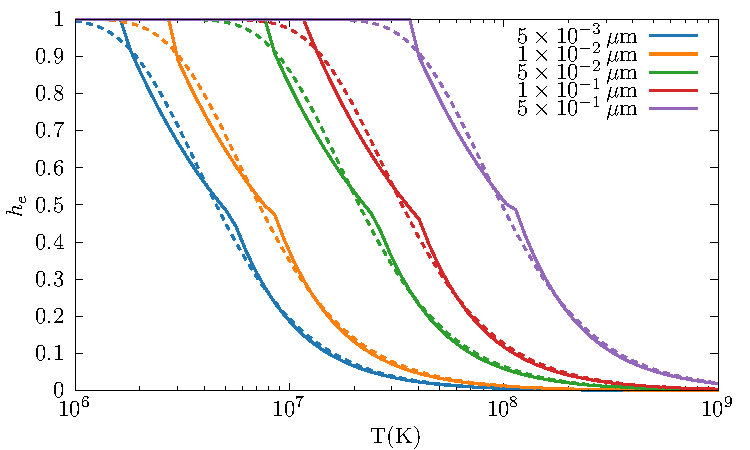
\includegraphics{assets/grain-transparency/grain-trans.pdf}
  \caption[Electron transparency method accuracy - $h_e$]{Grain transparency as a function of temperature for the estimate method described in equation \ref{eq:electrontransparencyestimate} (solid lines) and a 400 bin integration method (dashed lines).}
  \label{fig:graintransacc}
\end{figure}

\begin{figure}
  \centering
  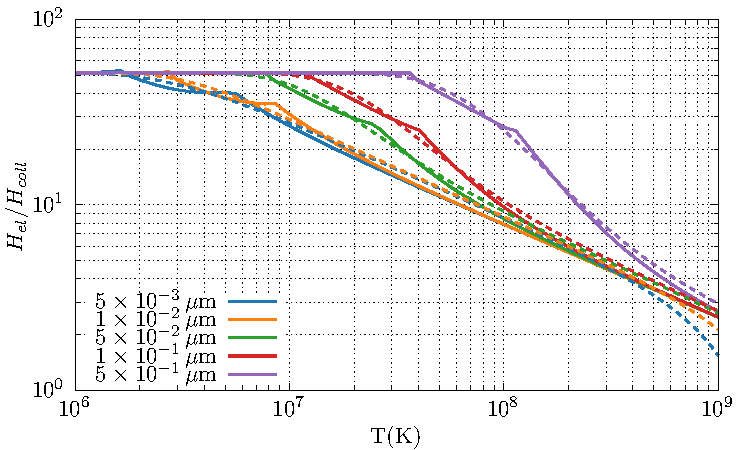
\includegraphics{assets/grain-transparency/contrib-comp.pdf}
  \caption[Electron transparency method accuracy - $H_{el}/H_{coll}$]{Comparison of the ratio heating rate of a dust grain due to incident electrons and incident atoms as a function of temperature for various grain sizes, whilst the result between the integration method and estimate method diverge, this is while the contribution of heating from electrons becomes less influential on the cooling rate of the grain.}
  \label{fig:contribution-int-vs-est}
\end{figure}

\begin{figure}
  \centering
  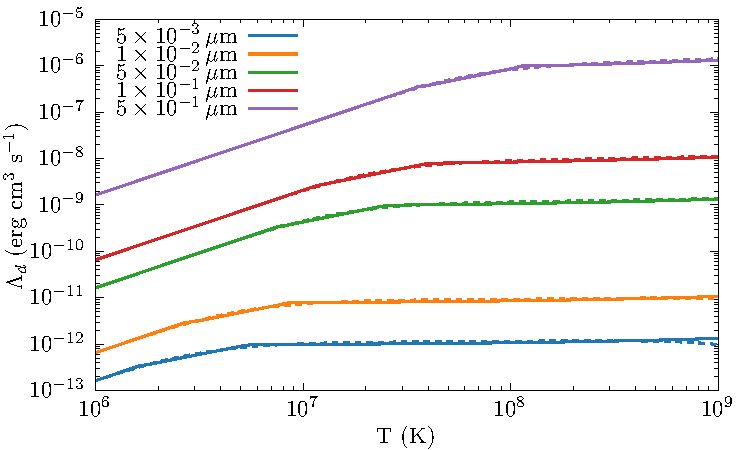
\includegraphics{assets/grain-transparency/lambda-comp.pdf}
  \caption[Electron transparency method accuracy - $\Lambda_d$]{$\Lambda_d$ as a function of temperature for various grain sizes, the estimate method is extremely close to the integral value aside from at the highest temperatures.}
  \label{fig:lambda-comp-int-vs-est}
\end{figure}



\begin{table}
  \centering
  \begin{tabular}{llll}
    \hline
    \multicolumn{1}{c}{\textbf{Method}} & \multicolumn{1}{c}{\textbf{t(s)}} & \multicolumn{1}{c}{\textbf{Iter/s}} & \multicolumn{1}{c}{\textbf{Speedup}} \\ \hline
    400 bin integration by parts & 36.03 & 35,526 & - \\
    Binary search + trilinear & 6.016 & 212,751 & 599\% \\
    Index calculation + bilinear + linear & 1.999 & 640,447 & 1,803\% \\
    \cite{dwek_infrared_1981} approximation & 0.147 & 8,693,171 & 24,510\% \\ \hline
  \end{tabular}
  \caption[Dust cooling calculation comparison]{Comparison of methods explored for estimating $\Lambda_d(\rho,a,T)$ in cooling code, $10^4$ initial values were chosen and 128 cooling sub-steps were performed, benchmark code was compiled and run using \texttt{GCC 10.3.0} with the \texttt{-O3} optimisation set on an Intel i7-7700HQ processor with a maximum clock speed of \SI{3.8}{\giga\hertz}.}
  \label{tab:electron-speedup}
\end{table}


% Compare accuracy and time taken
Table \ref{tab:electron-speedup} shows the improvements to performance inherent in the estimation method; the final result is that the approximation is over 24,500\% faster, the resulting dust cooling function therefore will have a minimal computational impact on the cooling loop as a whole.
As this approximation was conclusively shown to not significantly effect the cooling rate due to grain heating, the approximation was chosen.

Further improvements were made to correctly determine the electron number, $n_e$, to calculate the cooling contribution for dust due to grain-electron collisions.
the initial version of this code assumed that $n_e = 1.1 n_p$, an estimate based on solar abundances, however the electron-to-ion ratio varies significantly with temperature in a WC wind, which is hydrogen depleted and as such can vary from 0 to $\sim 4$ between \num{1e4} and \num{5e6} \si{\kelvin} (figure \ref{fig:electron-curve-no-elements}).
In order to solve this problem quickly for each timestep, a lookup table similar to the plasma cooling curves was used, containing the electron-ion ratio at temperatures between $10^4$ and $10^8$ \si{\kelvin} for each wind abundance.

\begin{figure}
  \centering
  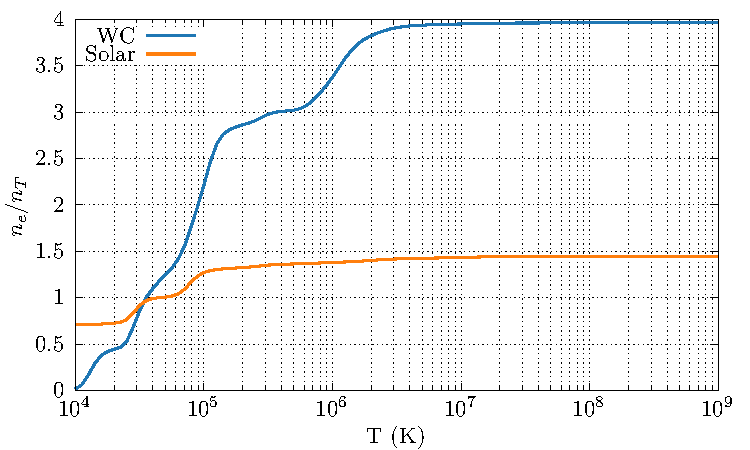
\includegraphics{assets/ionisation-fraction/ionisation-fraction-no-elements.pdf}
  \caption[Ionisation fraction for OB and WC stars]{Ionisation fraction}
  \label{fig:electron-curve-no-elements}
\end{figure}

%%//FIXME cooling loop schematic!

% Something along the line of This schematic describes, etc. etc. 
% Schematic

% This section needs more information, since this is very new to the codebase
\subsection{Exact cooling method}

%//TODO write this, you will have to ask Julian about this

\section{The BODMAS Advected Scalar Dust Model}
\label{sec:bodmas}

\section{Contemporary Dust Models}


\subsection{The Hendrix dust model}

Perhaps the most similar contemporary dust model is the model described in \cite{hendrix_pinwheels_2016} - as this model is concerned with simulating the dynamics of dust within a CWB.
This is not to say that these models are identical, of course, as the Hendrix model explores how dust spreads throughout the WCR of WR 98a, in order to compare with observational data using radiative transfer code. %//FIXME double check that one king 

% Differences between models 

The main differentiating factors between this model and our model are the driving mechanism and dust evolution.
In the Hendrix model dust is modelled as a separate fluid, with an Epstein drag function between the wind and dust fluids; this method allows for dust kinematics that aren't implicitly co-moving.
This is a more accurate method of modelling dust, however it requires significantly more processing time and is much more difficult to implement, requiring a numerical code that supports multiple fluids.
At the start of this PhD this was considered but eventually rejected due to time constraints.

The purpose of the Hendrix model is to analyse the distribution of dust within a CWB system, rather than to model the evolution of the dust itself.
To this end, the Hendrix model does not 

\section{Future dust models}



% Future work, adopt multi-fluid model?

% Mixing factors
The increased inertia of more massive dust grains could result in the kinematics of the dust flow diverging from the co-moving assumption.
To that end, a successor dust model would adopt a multi-fluid and drag function method, which was considered but not included for the sake of time.
